\textbf{Spatial pooling:} Using your \textbf{output feature map} in question 1, apply \textit{max-pooling} using a $[2 \times 2]$ kernel with a stride of 1. Recall from lecture that spatial pooling gives a CNN invariance to small transformations in the input, and max-pooling is more widely used over sum or average pooling due to empirically better performance. (2 pts)

\begin{figure}[H]
	\centering
	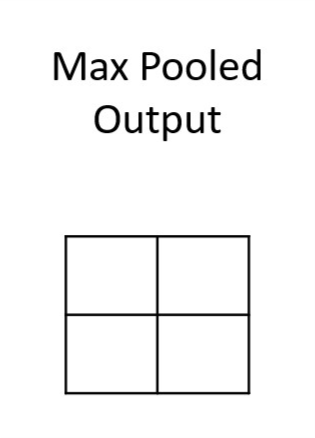
\includegraphics[width=.11\linewidth]{images/max_pooled_blank.png}
\end{figure}

\begin{tcolorbox}[title=Solution]
\end{tcolorbox}
